%%%%%%%% ICML 2023 EXAMPLE LATEX SUBMISSION FILE %%%%%%%%%%%%%%%%%

\documentclass{article}

% Recommended, but optional, packages for figures and better typesetting:
\usepackage{microtype}
\usepackage{graphicx}
\usepackage{subfigure}
\usepackage{booktabs} % for professional tables

\usepackage{tikz}
% Corporate Design of the University of Tübingen
% Primary Colors
\definecolor{TUred}{RGB}{165,30,55}
\definecolor{TUgold}{RGB}{180,160,105}
\definecolor{TUdark}{RGB}{50,65,75}
\definecolor{TUgray}{RGB}{175,179,183}

% Secondary Colors
\definecolor{TUdarkblue}{RGB}{65,90,140}
\definecolor{TUblue}{RGB}{0,105,170}
\definecolor{TUlightblue}{RGB}{80,170,200}
\definecolor{TUlightgreen}{RGB}{130,185,160}
\definecolor{TUgreen}{RGB}{125,165,75}
\definecolor{TUdarkgreen}{RGB}{50,110,30}
\definecolor{TUocre}{RGB}{200,80,60}
\definecolor{TUviolet}{RGB}{175,110,150}
\definecolor{TUmauve}{RGB}{180,160,150}
\definecolor{TUbeige}{RGB}{215,180,105}
\definecolor{TUorange}{RGB}{210,150,0}
\definecolor{TUbrown}{RGB}{145,105,70}

% hyperref makes hyperlinks in the resulting PDF.
% If your build breaks (sometimes temporarily if a hyperlink spans a page)
% please comment out the following usepackage line and replace
% \usepackage{icml2023} with \usepackage[nohyperref]{icml2023} above.
\usepackage{hyperref}


% Attempt to make hyperref and algorithmic work together better:
\newcommand{\theHalgorithm}{\arabic{algorithm}}

\usepackage[accepted]{icml2023}

% For theorems and such
\usepackage{amsmath}
\usepackage{amssymb}
\usepackage{mathtools}
\usepackage{amsthm}

% if you use cleveref..
\usepackage[capitalize,noabbrev]{cleveref}

%%%%%%%%%%%%%%%%%%%%%%%%%%%%%%%%
% THEOREMS
%%%%%%%%%%%%%%%%%%%%%%%%%%%%%%%%
\theoremstyle{plain}
\newtheorem{theorem}{Theorem}[section]
\newtheorem{proposition}[theorem]{Proposition}
\newtheorem{lemma}[theorem]{Lemma}
\newtheorem{corollary}[theorem]{Corollary}
\theoremstyle{definition}
\newtheorem{definition}[theorem]{Definition}
\newtheorem{assumption}[theorem]{Assumption}
\theoremstyle{remark}
\newtheorem{remark}[theorem]{Remark}

% Todonotes is useful during development; simply uncomment the next line
%    and comment out the line below the next line to turn off comments
%\usepackage[disable,textsize=tiny]{todonotes}
\usepackage[textsize=tiny]{todonotes}


% The \icmltitle you define below is probably too long as a header.
% Therefore, a short form for the running title is supplied here:
\icmltitlerunning{short title}

\begin{document}

\twocolumn[
\icmltitle{Title\\second line}

% It is OKAY to include author information, even for blind
% submissions: the style file will automatically remove it for you
% unless you've provided the [accepted] option to the icml2023
% package.

% List of affiliations: The first argument should be a (short)
% identifier you will use later to specify author affiliations
% Academic affiliations should list Department, University, City, Region, Country
% Industry affiliations should list Company, City, Region, Country

% You can specify symbols, otherwise they are numbered in order.
% Ideally, you should not use this facility. Affiliations will be numbered
% in order of appearance and this is the preferred way.
\icmlsetsymbol{equal}{*}

% authors
\begin{icmlauthorlist}
\icmlauthor{Vojtěch Sýkora}{equal,first}
\icmlauthor{Denis Kovačević}{equal,second}
\icmlauthor{Nam Nguyen The}{equal,third}
\end{icmlauthorlist}

% fill in your matrikelnummer, email address, degree, for each group member
\icmlaffiliation{first}{Matrikelnummer 6636502, vojtech.sykora@student.uni-tuebingen.de, MSc Machine Learning}
\icmlaffiliation{second}{Matrikelnummer 6707752, denis.kovacevic@student.uni-tuebingen.de, MSc Machine Learning}
\icmlaffiliation{third}{Matrikelnummer 6608479, nam.nguyen-the@student.uni-tuebingen.de, MSc Machine Learning}

% You may provide any keywords that you
% find helpful for describing your paper; these are used to populate
% the "keywords" metadata in the PDF but will not be shown in the document
\icmlkeywords{Machine Learning, ICML}

\vskip 0.3in
]

% this must go after the closing bracket ] following \twocolumn[ ...

% This command actually creates the footnote in the first column
% listing the affiliations and the copyright notice.
% The command takes one argument, which is text to display at the start of the footnote.
% The \icmlEqualContribution command is standard text for equal contribution.
% Remove it (just {}) if you do not need this facility.

%\printAffiliationsAndNotice{}  % leave blank if no need to mention equal contribution
\printAffiliationsAndNotice{\icmlEqualContribution} % otherwise use the standard text.

\begin{abstract}
    % Abstracts typically start
    % with a sentence motivating why the subject is in-
    % teresting. Then mention the data, methodology
    % or methods you are working with, and describe
    % results
    Code is available at \url{https://github.com/sykoravojtech/IHD_germany_2024}.

\end{abstract}

\section{Introduction}\label{sec:intro}
% Motivate the problem, situation or topic you decided to
% work on. Describe why it matters (is it of societal, eco-
% nomic, scientific value?). Outline the rest of the paper (use
% references, e.g. to Section 2: What kind of data you are
% working with, how you analyse it, and what kind of conclu-
% sion you reached. The point of the introduction is to make
% the reader want to read the rest of the paper.

% Motivate the problem, situation or topic you decided to work on.
This discrepancy, as highlighted in the analysis by 
\citet{Jasilionis2023} in "\textit{The underwhelming German life expectancy}," 
poses critical questions about the underlying factors contributing to this 
phenomenon.

% Describe why it matters (is it of societal, economic, scientific value?).


% Outline the rest of the paper (use references, e.g.~to \Cref{sec:methods}: 
% What kind of data you are working with, how you analyse it, and what kind of 
% conclusion you reached. The point of the introduction is to make the reader want 
% to read the rest of the paper.



\section{Data and Methods}\label{sec:methods}
% In this section, describe \emph{what you did}. Roughly speaking, explain what data you worked with, how or from where it was collected, 
% it's structure and size. Explain your analysis, and any specific choices you made in it. Depending on the nature of your project, 
% you may focus more or less on certain aspects. If you collected data yourself, explain the collection process in detail. 
% If you downloaded data from the net, show an exploratory analysis that builds intuition for the data, and shows that you know the data well. 
% If you are doing a custom analysis, explain how it works and why it is the right choice. If you are using a standard tool, 
% it may still help to briefly outline it. Cite relevant works. You can use the \verb|\citep| (whole citation in parenthesis) 
% and \verb|\citet| (only year in parenthesis) commands for this purpose \citep{mackay2003information}.



% SUBSECTION
\subsection{Cardiovascular Diseases data}\label{sec:cardiovascular_data}

In \figurename~\ref{Cardiovascular diseases over time} we can see that Germany has very high incidence and death rate of cardiovascular diseases. 
\begin{figure*}[h]
    \vskip 0.2in
    \centering
    \centerline{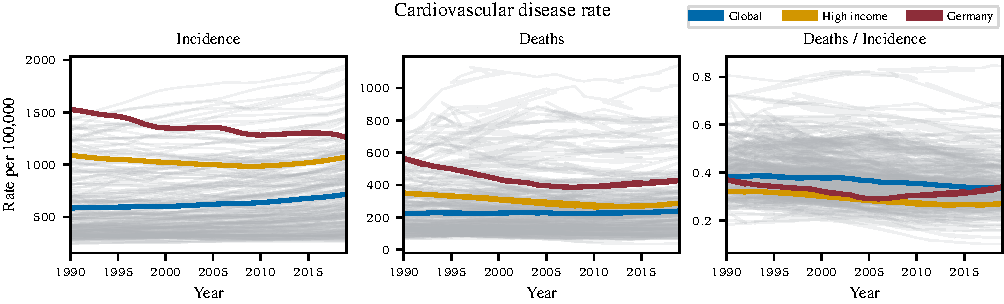
\includegraphics[]{fig/fig_cardiovascular_disease_rate.pdf}}
    \caption{Cardiovascular diseases in the world over time. From left to right: incidence rate, death rate, 
    and the ratio of death rate to incidence rate.}
    \label{Cardiovascular diseases over time}
\end{figure*}


\begin{table}[h]
    \centering
    \caption{Overview of the data sources. The missing data is calculated for the time period from 1990 to 2019.}
    \label{Data overview}
    \begin{tabular}{|c|c|c|c|}
    \hline
    Data source & No. of countries & Missing data\\
    \hline
    Ischemic heart disease & 206 & 0\%\\
    Health expenditure & 50 & 0\%\\
    Fat consumption & 194 & 0\%\\
    Alcohol consumption & 49 & 0\%\\
    Population age & 238 & 0\%\\
    \hline
    \end{tabular}
\end{table}



\section{Results}\label{sec:results}
% In this section outline your results. At this point, you are just stating the outcome of your analysis. 
% You can highlight important aspects (``we observe a significantly higher value of $x$ over $y$''), 
% but leave interpretation and opinion to the next section. This section absoultely \emph{has} to include at least two figures.

results

\section{Discussion \& Conclusion}\label{sec:conclusion}
% Use this section to briefly summarize the entire text. 
% Highlight limitations and problems, but also make clear statements where they are possible and supported by the analysis. 

discuss conclude

\section*{Contribution Statement}
% Explain here, in one sentence per person, what each group member contributed. 
% For example, you could write: Max Mustermann collected and prepared data. Gabi Musterfrau and John Doe performed the data analysis. 
% Jane Doe produced visualizations. All authors will jointly wrote the text of the report. 
% Note that you, as a group, a collectively responsible for the report. Your contributions should be roughly equal in amount and difficulty.
contribution

\bibliography{bibliography}
\bibliographystyle{icml2023}

\end{document}


% This document was modified from the file originally made available by
% Pat Langley and Andrea Danyluk for ICML-2K. This version was created
% by Iain Murray in 2018, and modified by Alexandre Bouchard in
% 2019 and 2021 and by Csaba Szepesvari, Gang Niu and Sivan Sabato in 2022.
% Modified again in 2023 by Sivan Sabato and Jonathan Scarlett.
% Previous contributors include Dan Roy, Lise Getoor and Tobias
% Scheffer, which was slightly modified from the 2010 version by
% Thorsten Joachims & Johannes Fuernkranz, slightly modified from the
% 2009 version by Kiri Wagstaff and Sam Roweis's 2008 version, which is
% slightly modified from Prasad Tadepalli's 2007 version which is a
% lightly changed version of the previous year's version by Andrew
% Moore, which was in turn edited from those of Kristian Kersting and
% Codrina Lauth. Alex Smola contributed to the algorithmic style files.



% chapter reference ... \Cref{sec:results}
% cite ... \citet \citep
% figure reference ... \figurename~\ref{Cardiovascular diseases over time} of \label{Cardiovascular diseases over time}